\paragraph{答:}
Java中的事件监听是整个Java消息传递的基础和关键。牵涉到三类对象:事件源(Event Source)、事件(Event)、事件监听器(Event Listener)。 

事件源是事件发生的场所,通常就是各个组件,它可以是一个按钮,编辑框等。 

事件监听者负责监听事件源所发生的事件,并对各种事件做出相应的响应。 

事件是描述事件源状态改变的对象。 

\begin{figure}[H]
	\centering
	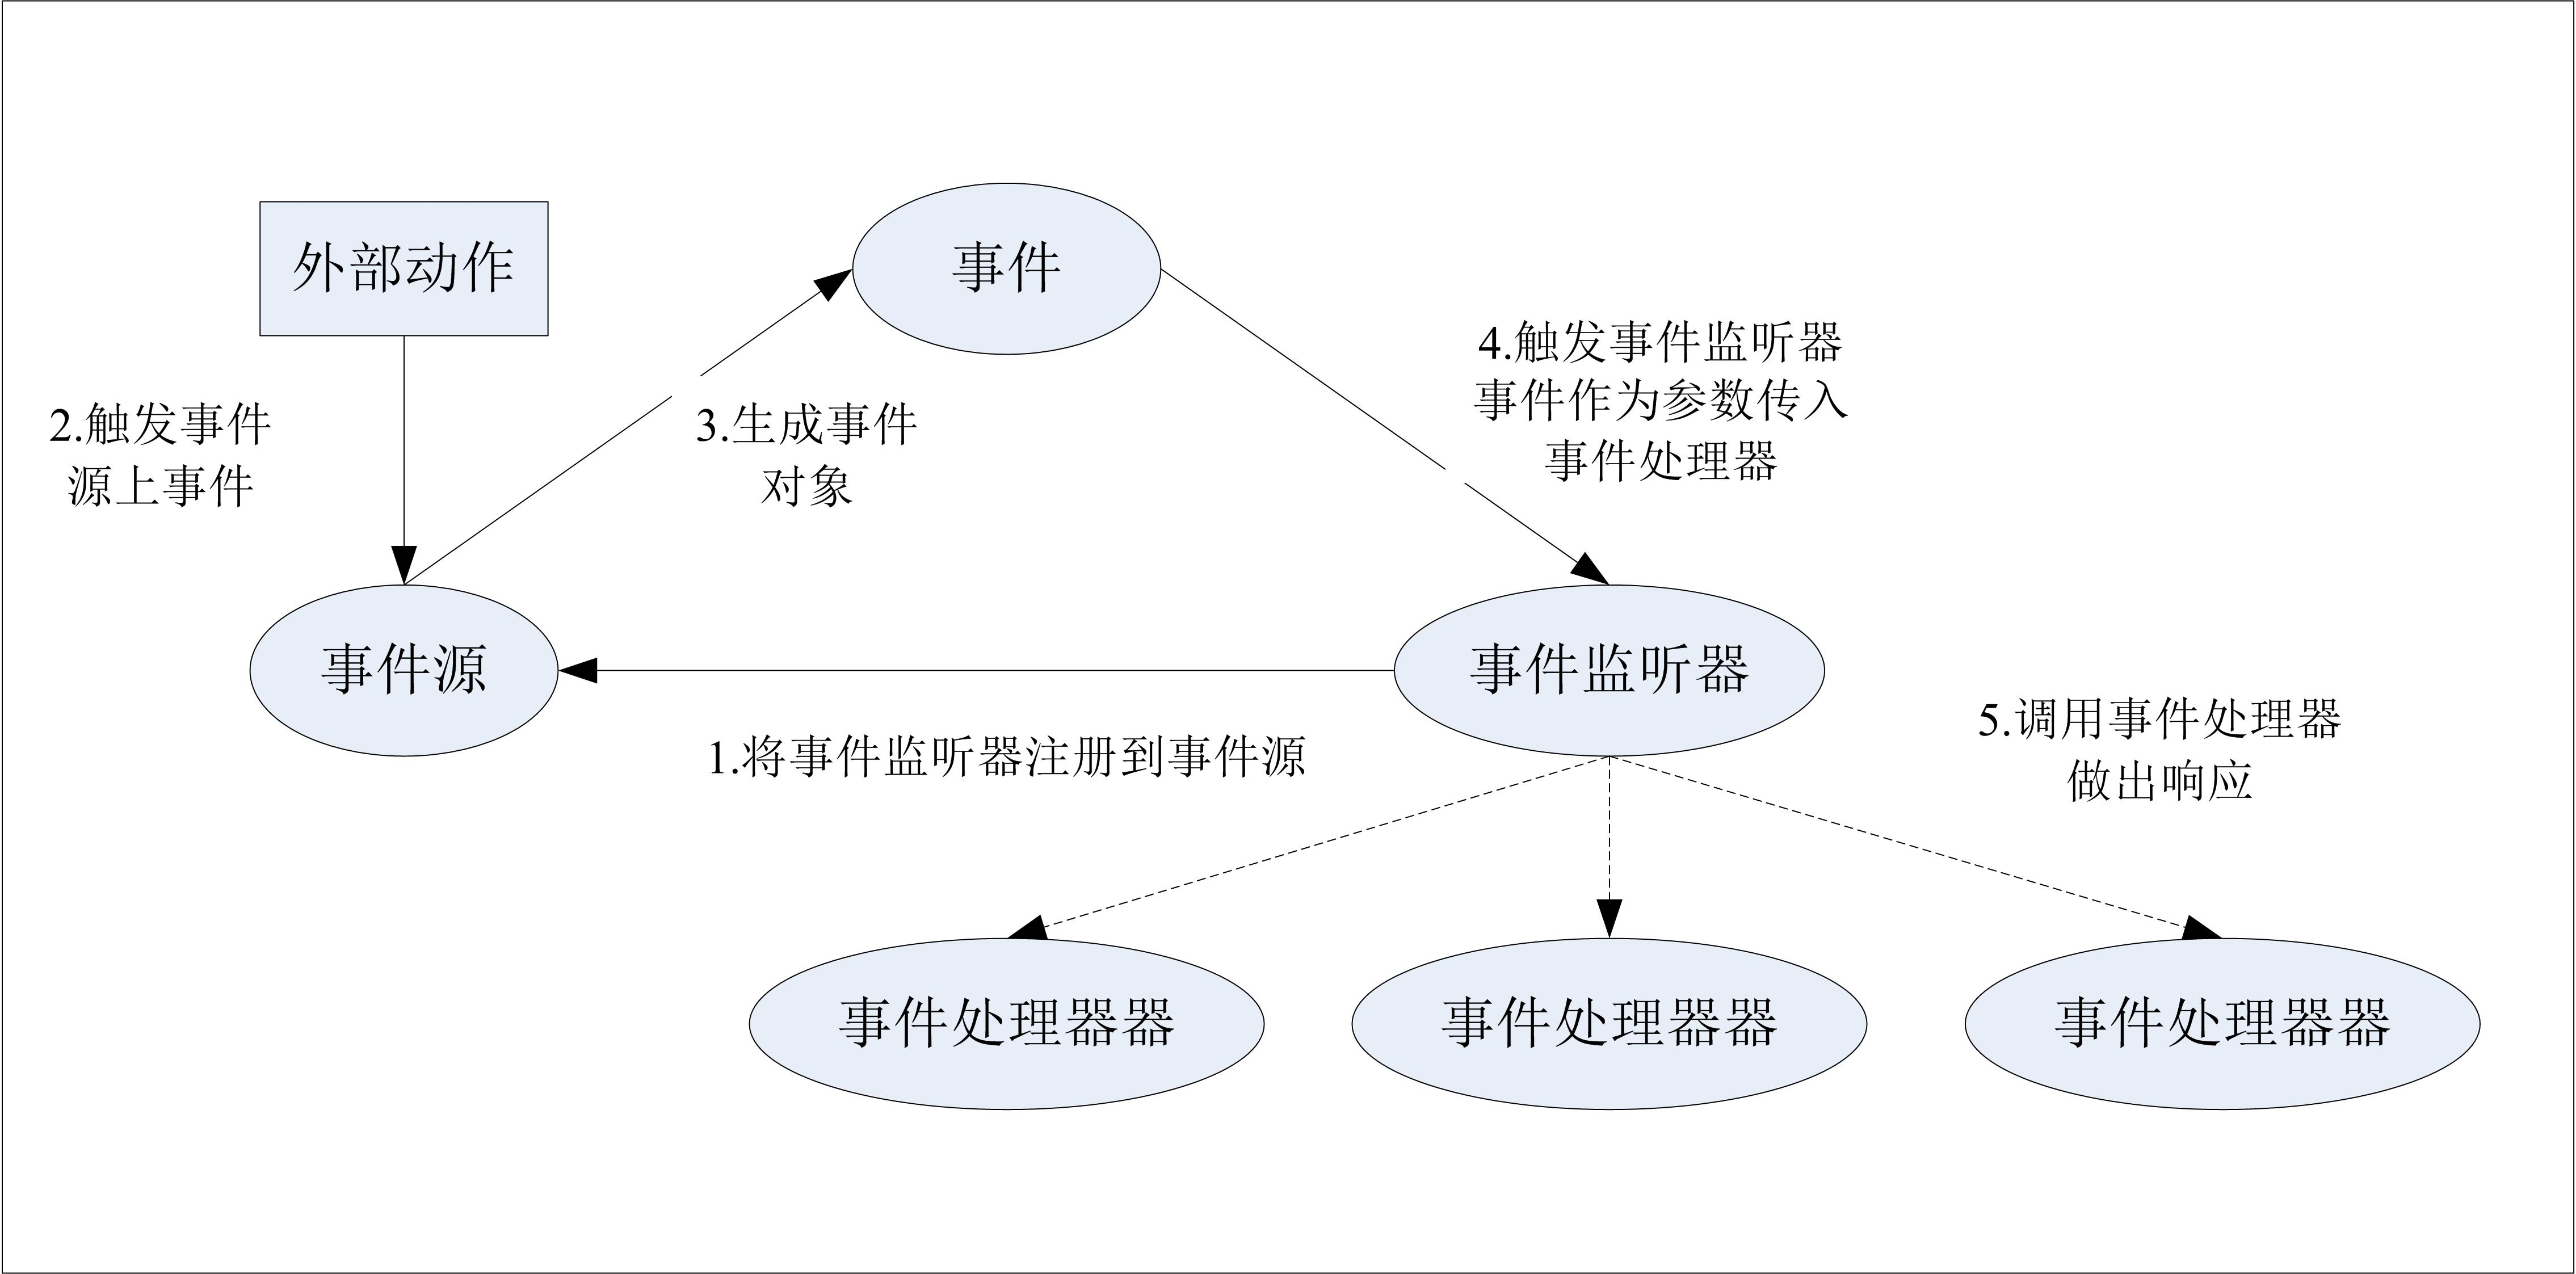
\includegraphics[width=\textwidth]{1.jpg}
	\caption{相互之间关系}
\end{figure}

其实现机制是先将一个监听器和一个监听对象绑定,当事件发生时,监听对象通知所有绑定了它的监听器,监听器收到消息后执行相应逻辑。正如以下时序图所示:

\begin{figure}[H]
	\centering
	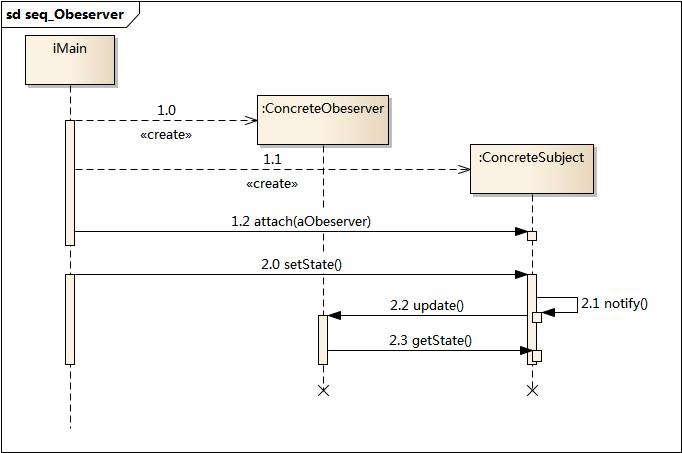
\includegraphics[width=\textwidth]{2.jpg}
	\caption{时序图}
\end{figure}

以之前写过的一个简单的计算器为例进行说明:
\begin{figure}[H]
	\centering
	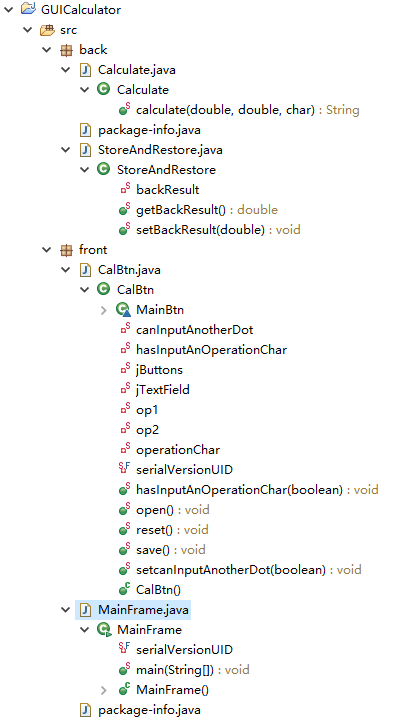
\includegraphics[height=0.9\textheight]{3.png}
	\caption{项目目录}
\end{figure}
以其中主框架MainFrame.java进行说明:

\begin{lstlisting}[language=java]
 package front;
 
 import static front.CalBtn.open;
 import static front.CalBtn.reset;
 import static front.CalBtn.save;
 
 import java.awt.BorderLayout;
 import java.awt.event.ActionEvent;
 import java.awt.event.ActionListener;
 
 import javax.swing.JFrame;
 import javax.swing.JMenu;
 import javax.swing.JMenuBar;
 import javax.swing.JMenuItem;
 import javax.swing.SwingUtilities;
 
 public class MainFrame extends JFrame {
 
 /**
 * 
 */
 private static final long serialVersionUID = -904161841520616291L;
 
 public static void main(String[] args) {
 // TODO Auto-generated method stub
 new MainFrame();
 }
 
 public MainFrame() {
 // TODO Auto-generated constructor stub
 SwingUtilities.invokeLater(new Runnable() {
 @Override
 public void run() {
 // TODO Auto-generated method stub
 setLayout(new BorderLayout(5, 5));
 JMenuBar jMenuBar = new JMenuBar();
 JMenu jMenuOpen = new JMenu("Options");
 jMenuBar.add(jMenuOpen);
 JMenuItem jMenuItemOpen = new JMenuItem("Open");
 JMenuItem jMenuItemSave = new JMenuItem("Save");
 JMenuItem jMenuItemReset = new JMenuItem("Reset");
 jMenuOpen.add(jMenuItemOpen);
 jMenuOpen.addSeparator();
 jMenuOpen.add(jMenuItemSave);
 jMenuOpen.addSeparator();
 jMenuOpen.add(jMenuItemReset);
 jMenuItemOpen.addActionListener(new ActionListener() {
 @Override
 public void actionPerformed(ActionEvent e) {
 // TODO Auto-generated method stub
 open();
 }
 });
 jMenuItemSave.addActionListener(new ActionListener() {
 @Override
 public void actionPerformed(ActionEvent e) {
 // TODO Auto-generated method stub
 save();
 }
 });
 jMenuItemReset.addActionListener(new ActionListener() {
 @Override
 public void actionPerformed(ActionEvent e) {
 // TODO Auto-generated method stub
 reset();
 }
 });
 setJMenuBar(jMenuBar);
 add(new CalBtn(), BorderLayout.CENTER);
 setTitle("Calculator");
 setSize(300, 500);
 setDefaultCloseOperation(JFrame.EXIT_ON_CLOSE);
 setLocationRelativeTo(null);
 setVisible(true);
 }
 });
 }
 } 
\end{lstlisting}
可以看到其中三个JButton(jMenuItemOpen, jMenuItemSave, jMenuItemReset)被添加上了ActionListener,以分别监听三个按钮的点击事件并执行相应逻辑。当这三个按钮被点击时,事件ActionEvent会通知相应的ActionListener然后执行ActionListenr下的actionPerformed内的逻辑,完成相应功能。